\documentclass[12pt,a4paper,final]{book}
\usepackage[utf8]{inputenc}
\usepackage{graphicx}
\usepackage[italian]{babel}
\usepackage[a4paper, headheight=15mm, width=150mm,top=25mm,bottom=25mm,bindingoffset=6mm]{geometry}
\usepackage{fancyhdr}
\usepackage{xcolor}
\usepackage{cite}
\usepackage[final]{pdfpages}
\definecolor{codegreen}{rgb}{0,0.6,0}
\definecolor{codegray}{rgb}{0.5,0.5,0.5}
\definecolor{codepurple}{rgb}{0.58,0,0.82}
\definecolor{backcolour}{rgb}{0.95,0.95,0.92}
\usepackage{listings}
\lstdefinestyle{mystyle}{
    commentstyle=\color{codegreen},
    keywordstyle=\color{magenta},
    numberstyle=\tiny\color{codegray},
    stringstyle=\color{codepurple},
    basicstyle=\ttfamily\footnotesize,
    breakatwhitespace=false,
    breaklines=false,
    captionpos=b,
    keepspaces=true,
    numbers=left,
    numbersep=5pt,
    showspaces=false,
    showstringspaces=false,
    showtabs=false,
    tabsize=2
}
\lstset{style=mystyle}
\pagestyle{fancy}
\fancyhf{}
\fancyhead[L]{\nouppercase{\leftmark}}
\fancyhead[R]{\thepage}
\linespread{1.1}
\usepackage{amsmath}
\usepackage{mathtools}
\usepackage{nccmath}
\usepackage{mathrsfs}
\usepackage{units} 
\usepackage{subcaption}
\usepackage{afterpage}
\usepackage[pdfa]{hyperref}
%%%%%%%%%%%%%%%%%%%%%%%%%%%%%%%%%%%%%%%%%%%%%%%%%%%%%%%%
\title{Tesi di laurea triennale di Eleonora Gatti}
\author{Eleonora Gatti}
\date{Maggio/Luglio 2020}
%%%%%%%%%%%%%%%%%%%%%%%%%%%%%%%%%%%%%%%%%%%%%%%%%%%%%%%
%%%%%%%%%%%%%%%%%%%%%%%%%%%%%%%%%%%%%%%%%%%%%%%%%%%%%%%
%%%%%%%%%%%%%%%%%%%%%%%%%%%%%%%%%%%%%%%%%%%%%%%%%%%%%%%

\begin{document}

%%%%%%%%%%%%%%%%%%%%  PRIMA PAGINA  %%%%%%%%%%%%%%%%%%%

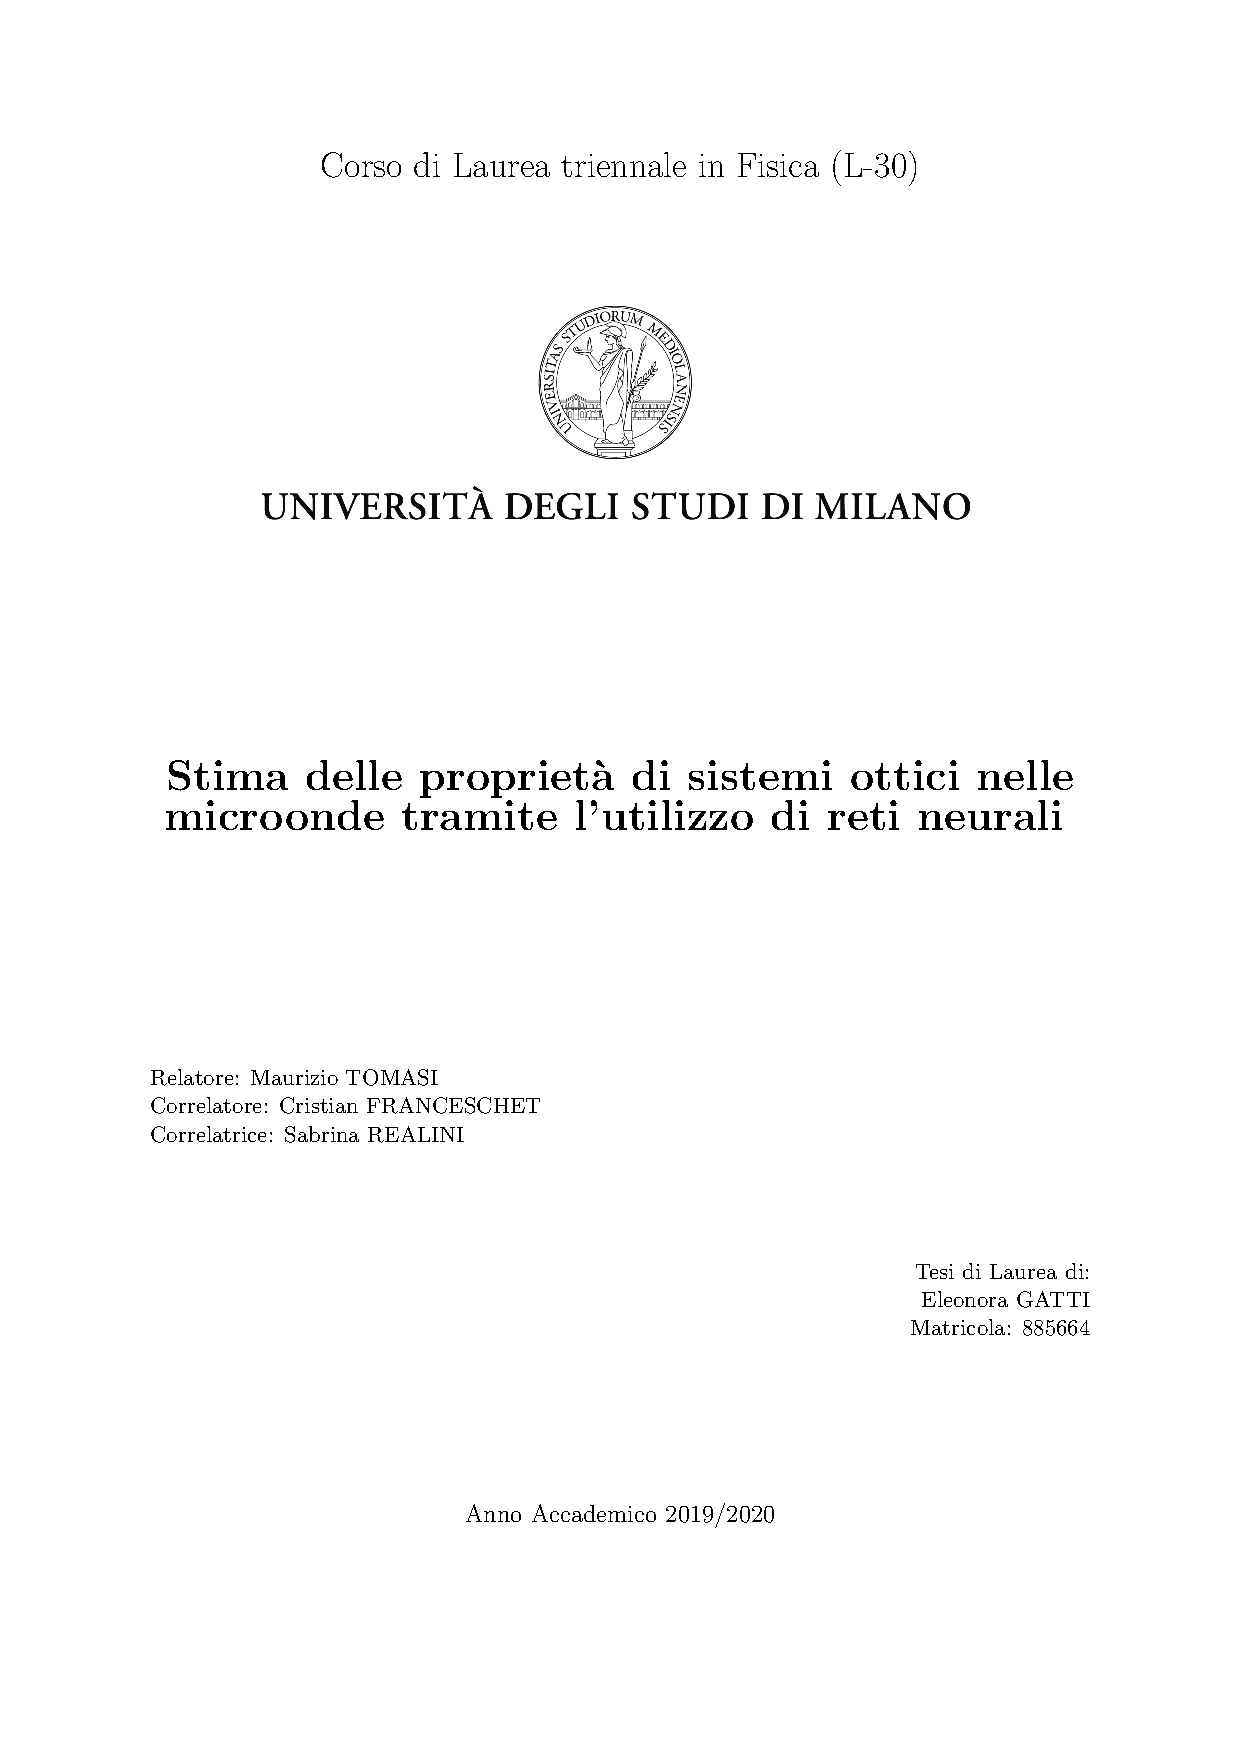
\includepdf[pages=-]{../frontespizio/frontespizio.pdf}
\newpage
\thispagestyle{empty}
\clearpage\mbox{}\clearpage
\newpage
\thispagestyle{empty}

%%%%%%%%%%%%%%%%%%%%%%%  INDICE  %%%%%%%%%%%%%%%%%%%%%

\tableofcontents
\newpage

%%%%%%%%%%%%%%%%%%%%  CAPITOLO 1  %%%%%%%%%%%%%%%%%%%%

\chapter{Sistemi ottici nelle microonde}\label{intro_sistemi_ottici}
Tutta l'informazione che abbiamo a disposizione su oggetti astronomici molto distanti è contenuta nella radiazione elettromagnetica emessa. Per secoli l'unico tipo di analisi possibile è stata quella nello spettro del visibile. Oggigiorno esistono svariate branche dell'astrofisica che analizzano segnali provenienti dall'Universo a diverse frequenze elettromagnetiche; una di queste branche riguarda lo studio del cosmo attraverso le microonde. 

    %%%%%%%%%%%%%%%%%%%  CAPITOLO 1.1  %%%%%%%%%%%%%%%%%%%

\section{Utilizzo delle microonde in astrofisica}\label{microonde_astrofisica}
Il range delle lunghezze d'onda delle microonde è $\lambda \sim 1 \unit{mm} \div 10 \unit{cm}$\footnote{Il confine tra onde radio e microonde non è netto, spesso si parla di radio estendendo il range di lunghezze d'onda anche a quello delle microonde.}. \\
\noindent \`E estremamente importante fare osservazioni a grandi lunghezze d'onda, nel millimetrico e oltre, poichè esistono numerosissime sorgenti cosmologiche che emettono in questo range e possono essere analizzate tramite sistemi ottici nelle microonde.
I segnali più comunemente studiati in radio astronomia e attraverso le microonde sono:
\begin{itemize}
	\item Radiazione emessa da gas ionizzato;
	\item Radiazione di sincrotrone, dovuta al moto di particelle cariche libere di muoversi nell'Universo e deviate da campi magnetici;
	\item Effetto Sunyaev-Zeldovich, che permette di rivelare ammassi di galassie altrimenti non visibili;
	\item Emissioni del Sole;
	\item Radiazioni da regioni $H_{II}$, si tratta di regioni nello spazio in cui sono presenti stelle molto calde (di tipo O o di tipo B) che ionizzano il gas intorno ad esse il quale emette nelle microonde e nel radio;
	\item Supernovae e resti di Supernovae\footnote{La Crab Nebula, per esempio, è estremamente visibile nelle moicroonde.};
	\item Pulsar;
	\item Radio galassie;
	\item CMB.
\end{itemize}
La \textbf{CMB}, Cosmic Microwave Background, è la radiazione a microonde di fondo cosmico che permea l’intero Universo.
Secondo il \textit{Modello Cosmologico Standard (SCM)} l'Universo ha avuto origine circa $14$ miliardi di anni fa da una singolarità iniziale: il \textit{Big Bang}. \\
\noindent Nei primissimi istanti dopo il \textit{Big Bang} vi fu una rapidissima fase di espansione ($10^{-33}~\unit{s}$), detta \textit{inflazione}, seguita da un'espansione più lenta e regolare, che continua tutt'ora. Inizialmente materia e radiazione erano in equilibrio in un plasma estremamente caldo; la progressiva espansione ha causato un abbassamento della temperatura del plasma. L'equilibrio tra materia e radiazione venne a mancare quando la temperatura raggiunse $T \simeq 3000~\unit{K}$. Questo causò il \textit{disaccoppiamento} tra materia e radiazione: la maggior parte degli elettroni venne catturata dai nuclei atomici permettendo la formazione dei primi atomi neutri. Convenzionalmente si considera come tempo al quale si è verificato il \textit{disaccoppiamento} tra materia e radiazione l'istante $t_{dec}$ in cui il libero cammino medio dei fotoni divenne maggiore della scala dell'Universo osservabile. Questo accadde a circa $380~000~\unit{anni}$ dal \textit{Big Bang} e da allora i fotoni primordiali sono liberi di vagare nello spazio e sono i responsabili della radiazione a microonde di fondo cosmico. \\
\newline
Data la vastità di campi in cui può essere effettuato uno studio nelle microonde, è di fondamentale importanza avere a disposizione un sistema ottico che permetta questo tipo di analisi. In particolare è necessario riconoscere la direzione dalla quale un determinato segnale microonde proviene.

    %%%%%%%%%%%%%%%%%%%  CAPITOLO 1.2  %%%%%%%%%%%%%%%%%%%
\section{Diagramma di radiazione}\label{rad_pattern}
Un sistema ottico è un dispositivo il cui scopo è quello di registrare la luce proveniente dal cielo e mandarla ad un rivelatore.
La risposta di un sistema ottico ideale può essere rappresentata come una delta di Dirac: non nulla solo lungo la linea di vista.
Tuttavia i fenomeni di interferenza e diffrazione rendono la situazione molto più complessa; in particolare nella radio astronomia e nell'astronomia a microonde il problema è particolarmente importante poichè le dimensioni degli elementi ottici degli strumenti sono comparabili alle lunghezze d'onda d'interesse.

\begin{figure}[!ht]
\centering
	\begin{subfigure}{0.5\textwidth}
	    \centering
	    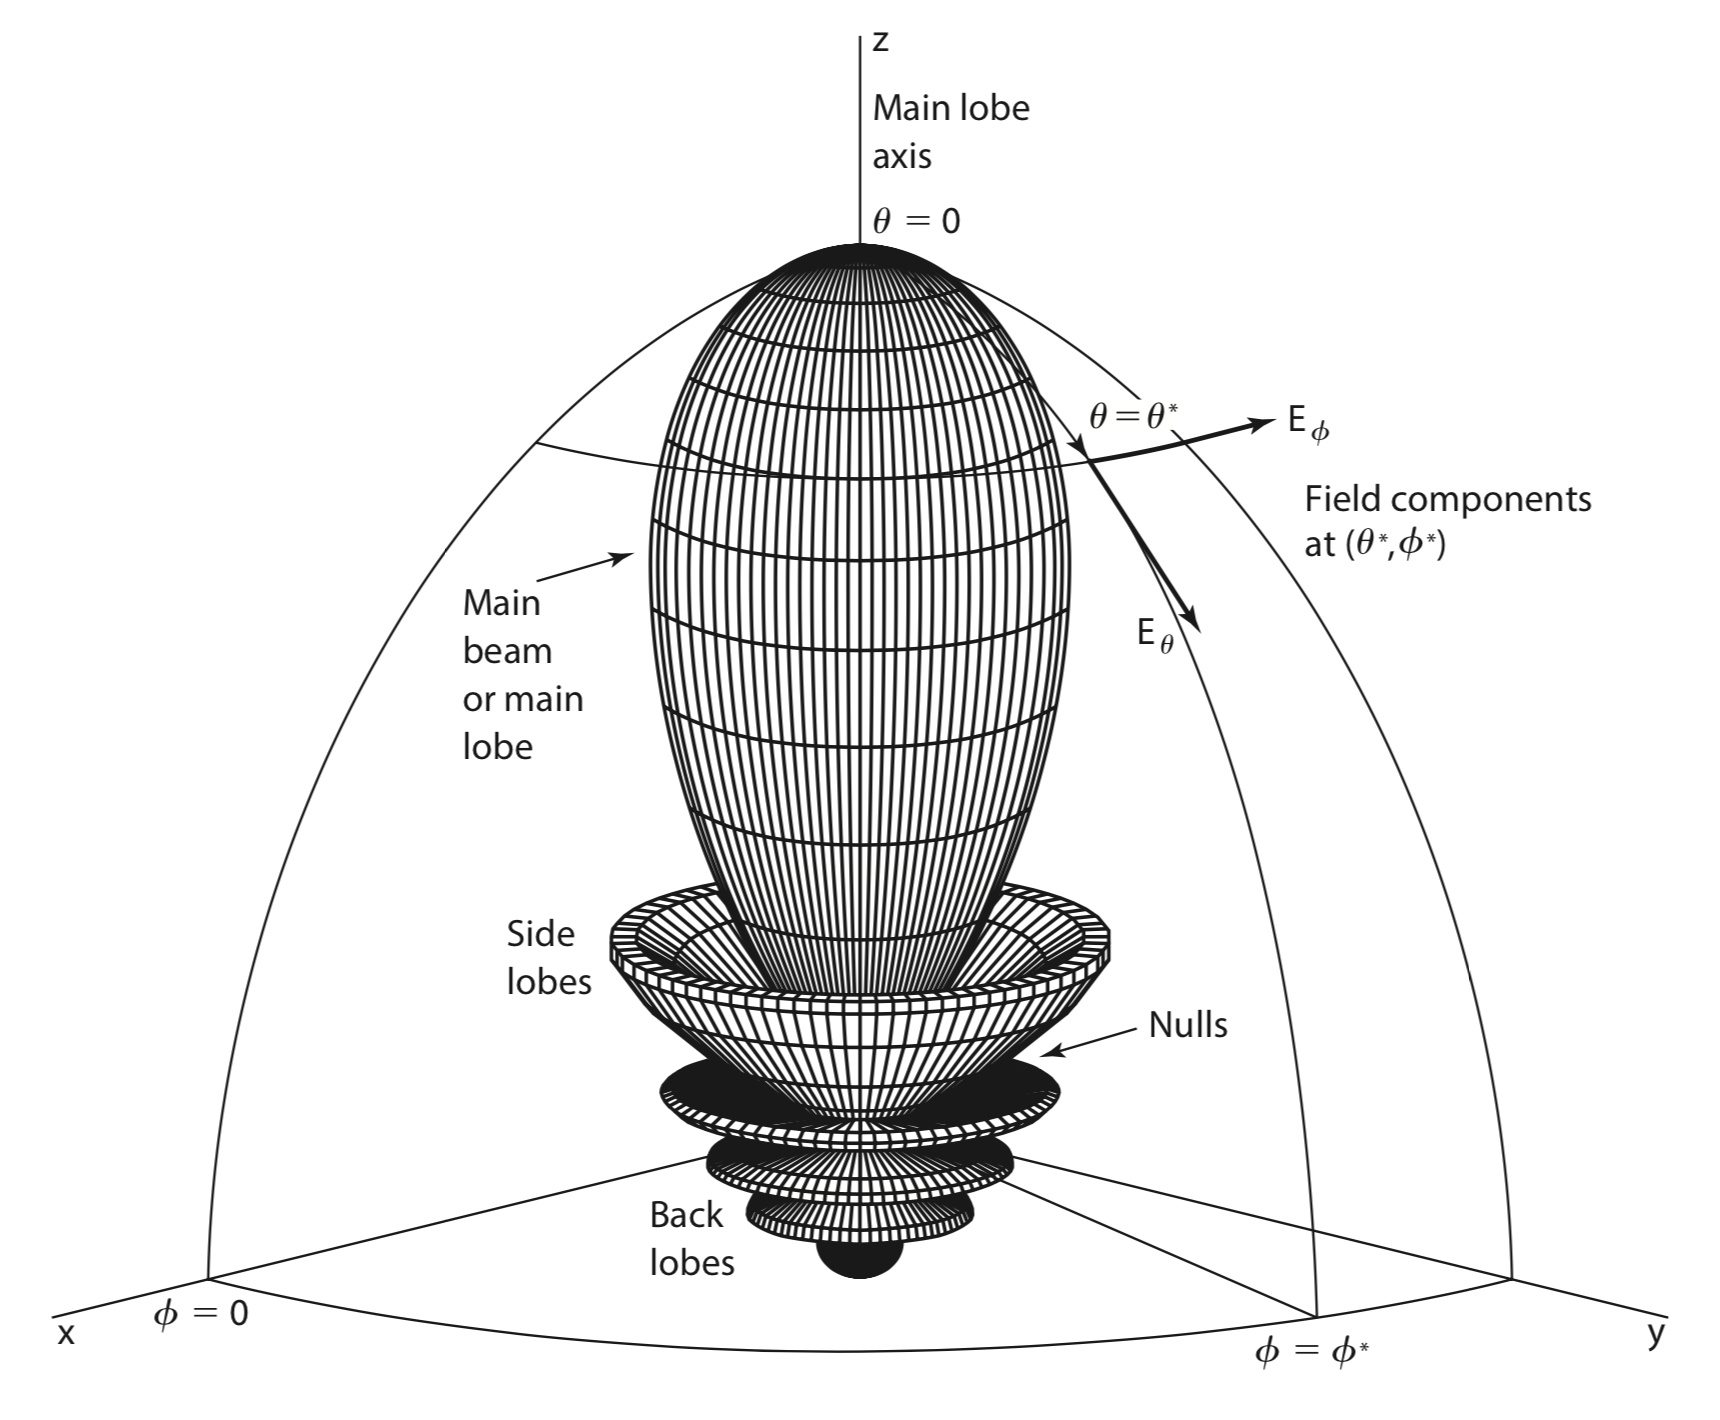
\includegraphics[width=\linewidth]{../figures/diag_rad}
	    \caption{}
	    \label{beam}
	\end{subfigure}
	\begin{subfigure}{0.45\textwidth}
		\centering
	    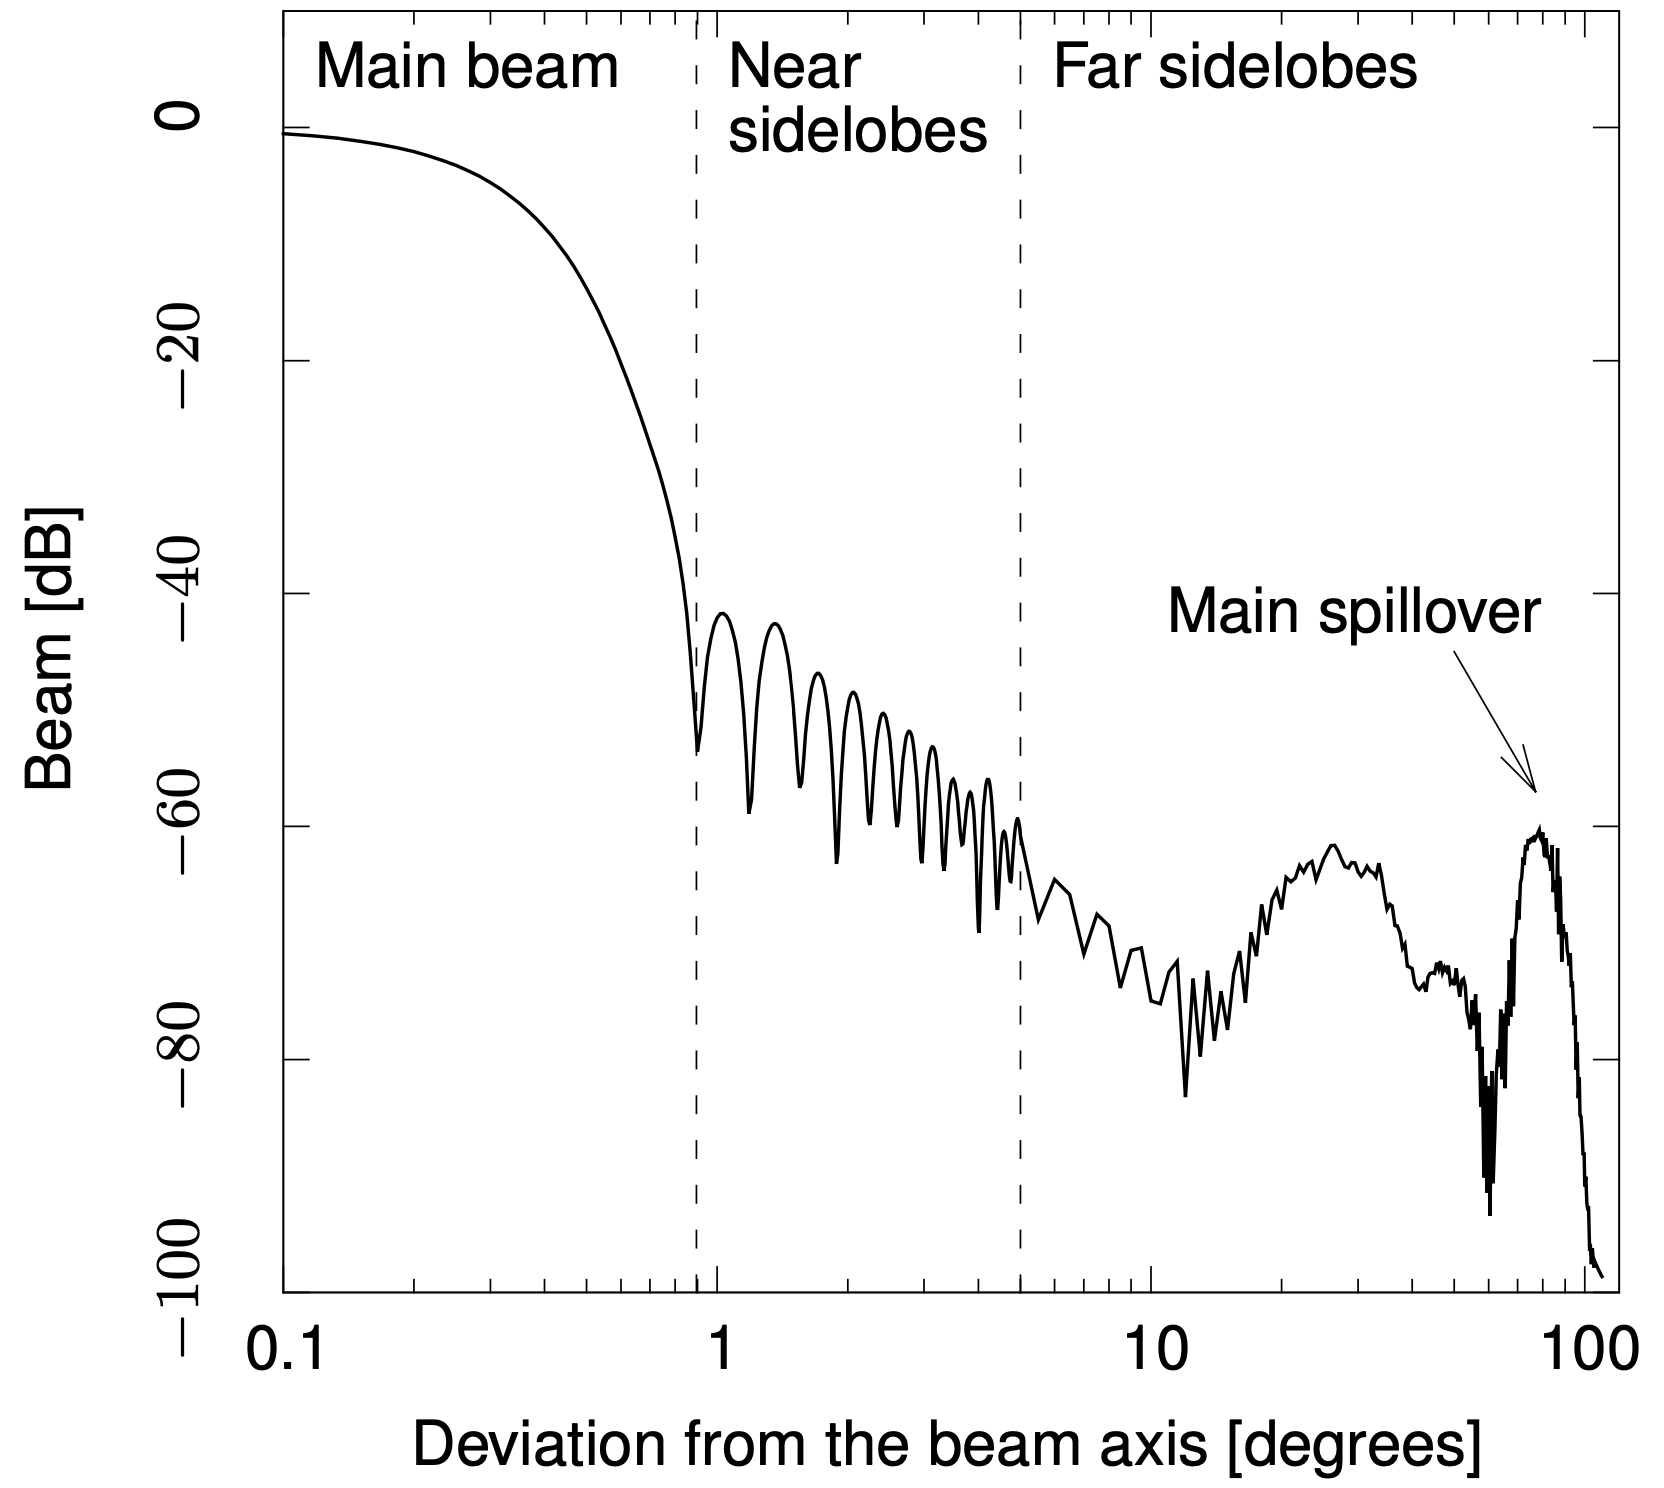
\includegraphics[width=\linewidth]{../figures/risposta_ottica.png}
		\caption{}
		\label{beam_cut}
	\end{subfigure}
\caption{Tipico andamento della \textit{beam function} $\gamma(\theta,\phi)$. La Fig.~\ref{beam} rappresenta il diagramma di radiazione tridimensionale di un'antenna direzionale.\cite{cmb}. La Fig.~\ref{beam_cut} rappresenta una sezione dello stesso grafico su un piano parallelo all'asse del main lobe.\cite{planck}}
\label{diag_rad}
\end{figure}

La risposta angolare di un sistema ottico è quantificata da una funzione $\gamma(\theta,\phi)$ detta \textit{beam function} che definisce il \textbf{diagramma di radiazione}. Idealmente $\gamma(\theta,\phi)$ dovrebbe corrispondere a una delta di Dirac\footnote{Questa idealizzazione viene spesso chiamata \textit{pencil beam idealization}}, quello che viene in realtà osservato è una risposta simile a quella riportata in Fig.~\ref{diag_rad}.
\`E possibile osservare la presenza di un \textit{main beam} e di lobi secondari. Tipicamente la maggior parte della radiazione è contenuta nel main beam. \\
A partire dal diagramma di radiazione si definiscono alcuni parametri che permettono una sua descrizione; tali parametri sono i protagonisti di questo lavoro di tesi.
La \textbf{Full Width Half Maximum} (FWHM) del main beam è la larghezza angolare a metà della sua altezza ed è uno dei parametri più importanti e più diffusi per la caratterizzazione della risoluzione di uno strumento. Nel corso dei prossimi capitoli verranno considerati due diversi valori per la FWHM, rispetto all'asse $x$ e rispetto all'asse $y$. Attraverso queste due grandezze è possibile definire un ulteriore parametro: l'\textbf{ellitticità}. Questa è definita come il rapporto tra le due FWHM ponendo al numeratore la più grande tra FWHM$_x$ e FWHM$_y$.\\
Hanno inoltre grande importanza i parametri che riguardano la polarizzazione. Supponiamo di studiare un'antenna in trasmissione\footnote{Strumenti ottici per lo studio della CMB lavorano in ricezione ma è possibile studiare alternativamente un'antenna in trasmissione per il \textit{principio di reciprocità}.} e considerare una radiazione polarizzata. Fissiamo una direzione di polarizzazione; è allora possibile definire, rispetto a tale direzione, una componente \textit{co-polare} ed una componente \textit{cross-polare} della radiazione. La componente co-polare è data dalla frazione di radiazione con polarizzazione parallela alla direzione fissata mentre la componente cross-polare è data dalla frazione di radiazione con polarizzaizione perpendicolare a quella fissata. In particolare i parametri utilizzati nei prossimi capitoli riguardano la componente \textbf{co-polare massima} e la componente \textbf{cross-polare massima}.


    %%%%%%%%%%%%%%%%%%  CAPITOLO 1.3  %%%%%%%%%%%%%%%%%%%%

\section{Simulazione di sistemi ottici}\label{simulazioni}
Simulare un sistema ottico significa studiare quanta potenza viene ricevuta in funzione dell'angolo. Tipicamente per simulare la risposta angolare di un sistema ottico si usa il sofware \textit{GRASP} (General Reflector Antenna Software Package). Attraverso GRASP è stato possibile ottenere la tabella in Fig.~\ref{dataset} che riporta le caratteristiche del beam data una posizione $(x, y, z)$ sulla superficie focale.

\begin{figure}[!ht]
	\centering
	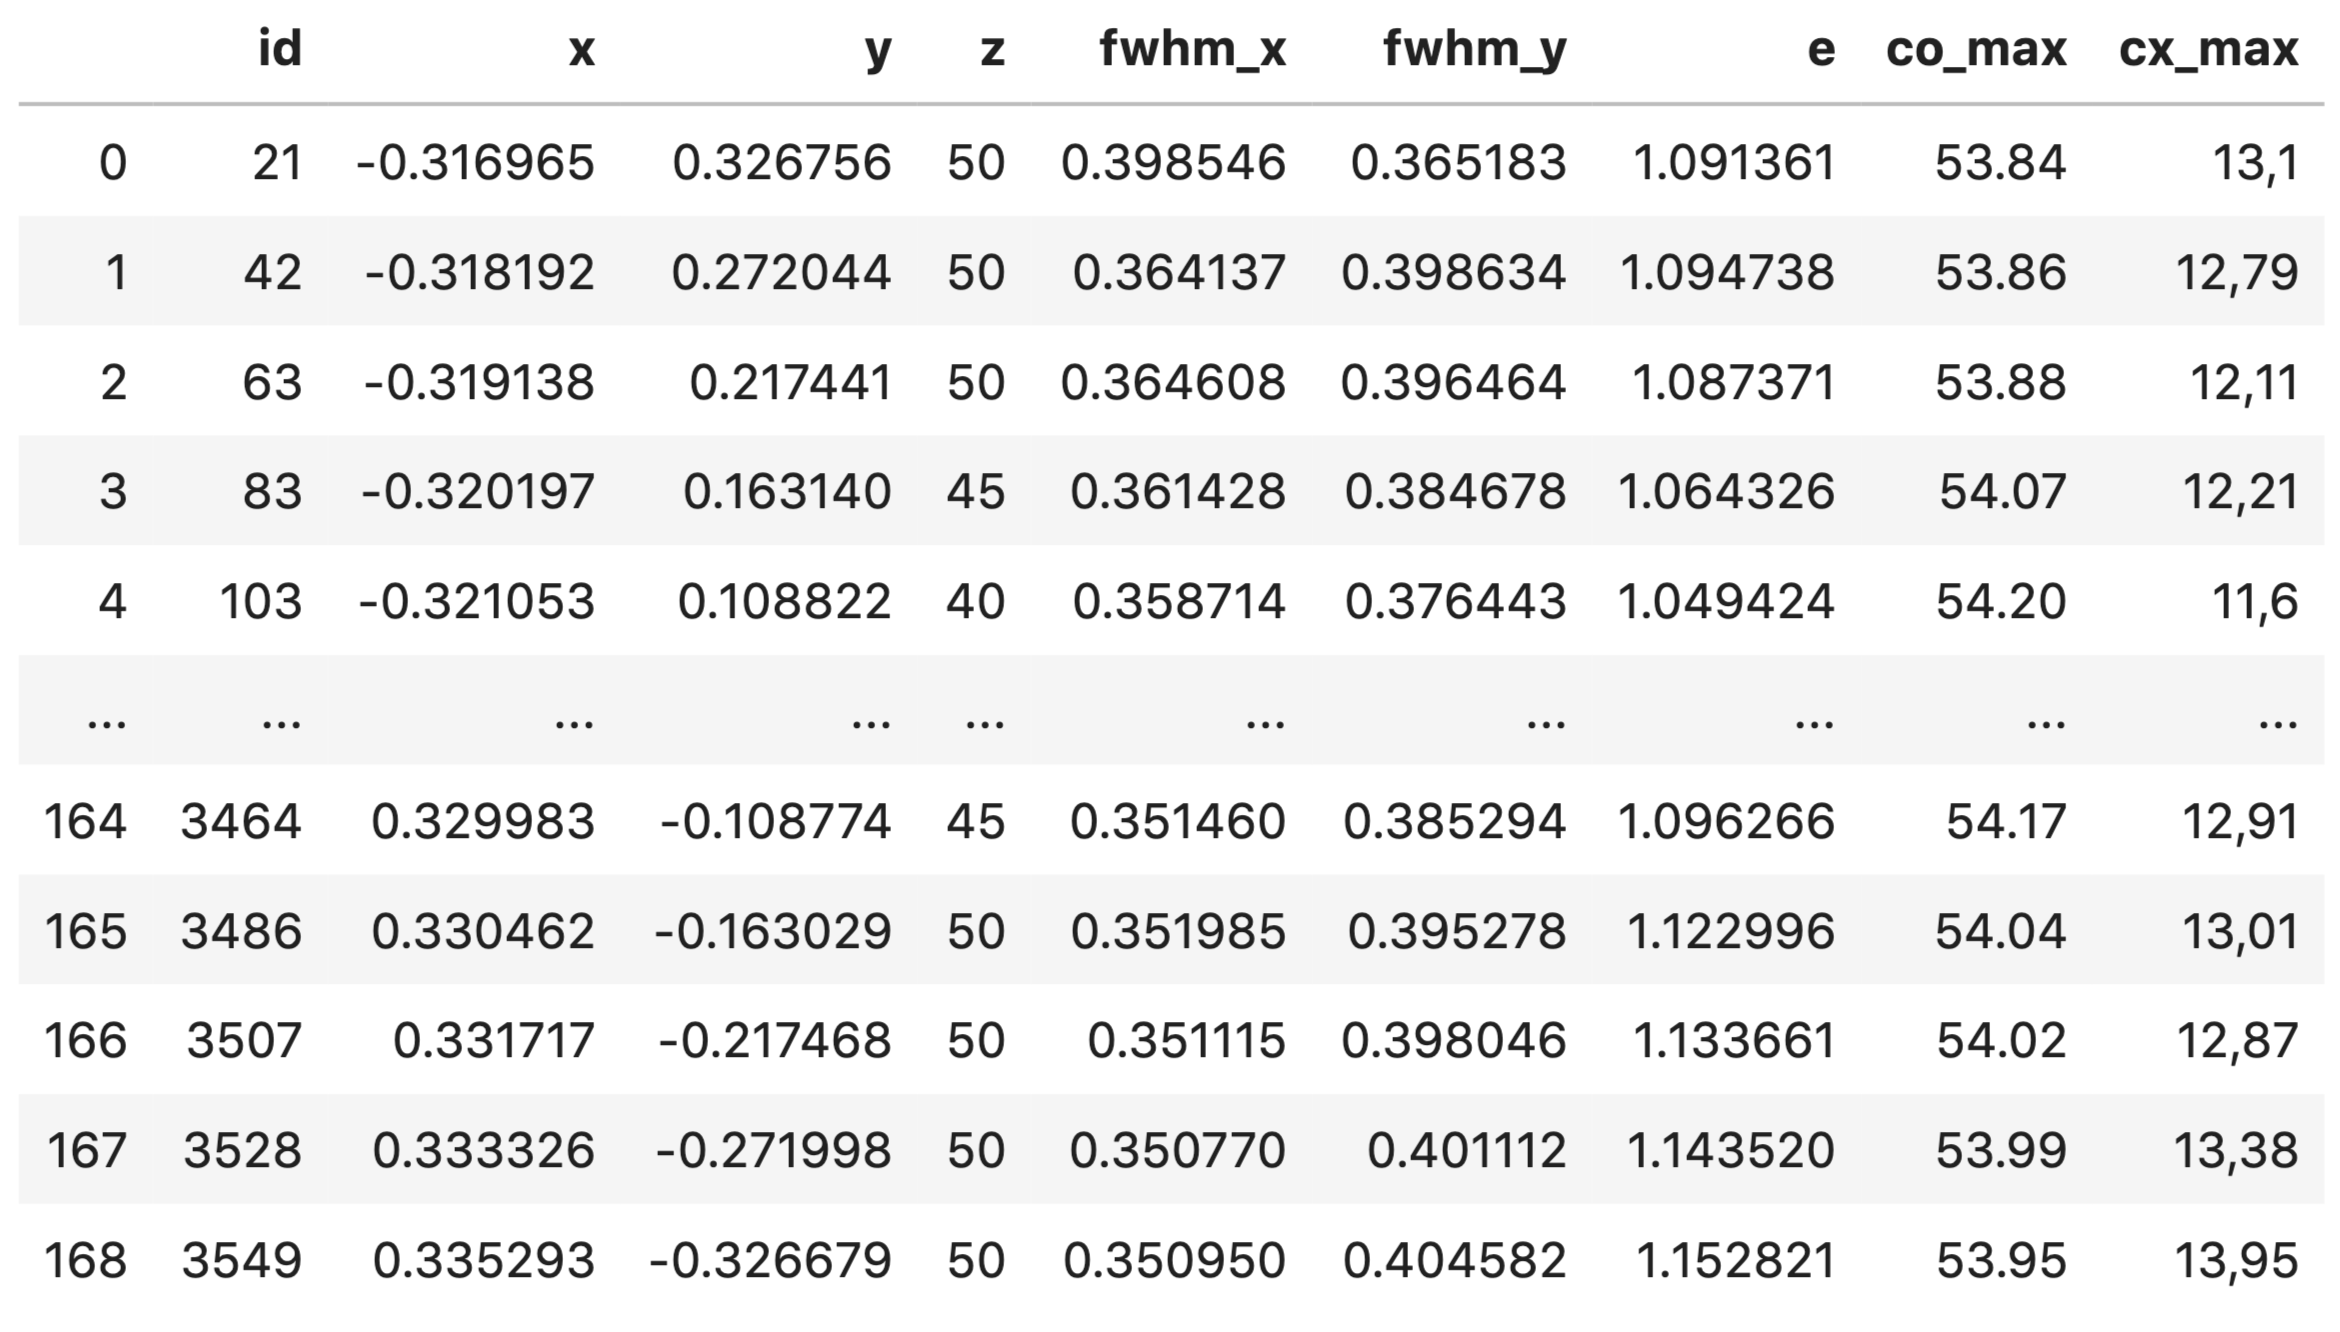
\includegraphics[width=0.8\linewidth]{../figures/dataset.png}
	\caption{Dataset relativo allo strumento STRIP ottenuto tramite la simulazione in GRASP. Tale dataset è stato utilizzato per l'analisi descritta nei capitoli successivi.}
	\label{dataset}
\end{figure}

GRASP è uno strumento molto potente che permette di simulare sistemi ottici complessi.
Tuttavia i tempi di calcolo di GRASP sono elevati\footnote{Per produrre i dati in Fig.~\ref{dataset} sono stati impiegati due giorni.}; per ogni simulazione, e quindi per ogni antenna, vengono costruiti dei grafici come quelli riportati in Fig.~\ref{beam_grasp} e poi da quelli vengono ricavati i valori riportati nel dataset ~\ref{dataset}. \\

Nel caso di STRIP è ancora possibile simulare l'intera ottica tramite GRASP poichè il numero di antenne è piuttosto limitato. Tuttavia per sistemi ottici più complessi in cui il numero di antenne diventa di circa 2 ordini di grandezza superiore, risulta del tutto impossibile effettuare una simulazione completa dell'intera ottica. \\
\noindent \`E quindi nata la necessità di trovare una via alternativa che permetta di stimare i parametri che descrivono il beam in una qualsiasi posizione.

\begin{figure}[!ht]
\centering
	\begin{subfigure}{0.49\textwidth}
	    \centering
	    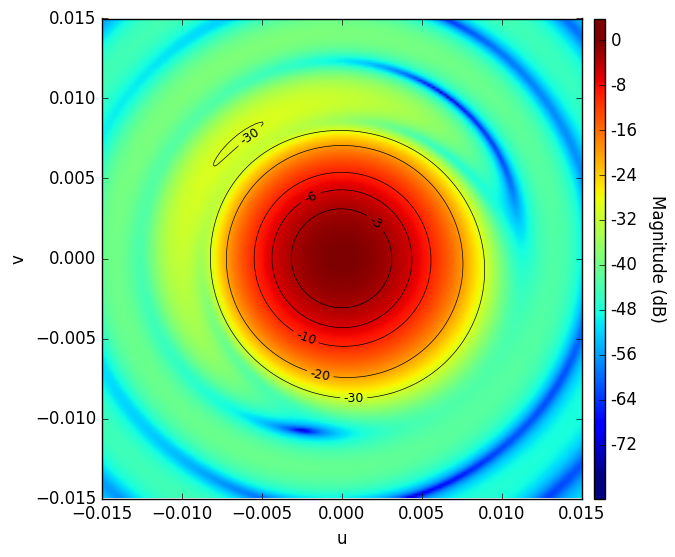
\includegraphics[width=\linewidth]{../figures/off-axis_co.png}
	    \caption{}
	    \label{off_axis_co}
	\end{subfigure}
	\begin{subfigure}{0.49\textwidth}
		\centering
	    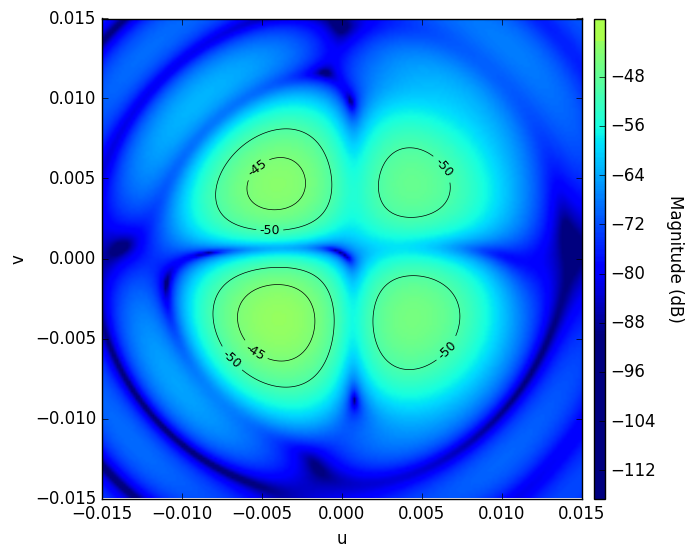
\includegraphics[width=\linewidth]{../figures/off-axis_cx.png}
		\caption{}
		\label{off_axis_cx}
	\end{subfigure}
\caption{Diagramma della componente co-polare~\ref{off_axis_co} e della componente cross-polare~\ref{off_axis_cx} di un'antenna off-axis. \`E possibile notare come il profilo del beam sia leggermente ellittico; per il sistema ottico di STRIP infatti l'ellitticità del fascio aumenta spostandosi dal centro del piano focale.}
\label{beam_grasp}
\end{figure}


%%%%%%%%%%%%%%%%%%%%%%%%%%%%%%%%%%%%%%%%%%%%%%%%%%%%%%%
%%%%%%%%%%%%%%%%%%%%%%%%%%%%%%%%%%%%%%%%%%%%%%%%%%%%%%%
%%%%%%%%%%%%%%%%%%%%%%%%%%%%%%%%%%%%%%%%%%%%%%%%%%%%%%%
%                   FINE CAPITOLO 1                   %
%%%%%%%%%%%%%%%%%%%%%%%%%%%%%%%%%%%%%%%%%%%%%%%%%%%%%%%
%%%%%%%%%%%%%%%%%%%%%%%%%%%%%%%%%%%%%%%%%%%%%%%%%%%%%%%
%%%%%%%%%%%%%%%%%%%%%%%%%%%%%%%%%%%%%%%%%%%%%%%%%%%%%%%


%%%%%%%%%%%%%%%%%%%%  CAPITOLO 2  %%%%%%%%%%%%%%%%%%%%

\chapter{Regressione con reti neurali}\label{reg_nn}

	%%%%%%%%%%%%%%%%%%%  CAPITOLO 2.1  %%%%%%%%%%%%%%%%%%%

\section{Machine learning e tipi di rete}

	%%%%%%%%%%%%%%%%%%%  CAPITOLO 2.2  %%%%%%%%%%%%%%%%%%%

\section{Struttura di una rete neurale}



%%%%%%%%%%%%%%%%%%%%%%%%%%%%%%%%%%%%%%%%%%%%%%%%%%%%%%%
%%%%%%%%%%%%%%%%%%%%%%%%%%%%%%%%%%%%%%%%%%%%%%%%%%%%%%%
%%%%%%%%%%%%%%%%%%%%%%%%%%%%%%%%%%%%%%%%%%%%%%%%%%%%%%%
%                   FINE CAPITOLO 2                   %
%%%%%%%%%%%%%%%%%%%%%%%%%%%%%%%%%%%%%%%%%%%%%%%%%%%%%%%
%%%%%%%%%%%%%%%%%%%%%%%%%%%%%%%%%%%%%%%%%%%%%%%%%%%%%%%
%%%%%%%%%%%%%%%%%%%%%%%%%%%%%%%%%%%%%%%%%%%%%%%%%%%%%%%


%%%%%%%%%%%%%%%%%%%%  CAPITOLO 3  %%%%%%%%%%%%%%%%%%%%

\chapter{Previsione delle proprietà di un diagramma di radiazione}\label{prev_param}

    %%%%%%%%%%%%%%%%%%%  CAPITOLO 3.1  %%%%%%%%%%%%%%%%%%%

\section{Interpolazione}\label{interpolazione}

         %%%%%%%%%%%%%%%%%%%  CAPITOLO 3.1.1  %%%%%%%%%%%%%%%%%%%

\subsection{Interp2d}\label{interp2d}

         %%%%%%%%%%%%%%%%%%%  CAPITOLO 3.1.2  %%%%%%%%%%%%%%%%%%%

\subsection{Curve Fit}\label{curve_fit}

        %%%%%%%%%%%%%%%%%%%  CAPITOLO 3.1.3  %%%%%%%%%%%%%%%%%%%

\subsection{Risultati dell'interpolazione}\label{risultati_interpolazione}


     %%%%%%%%%%%%%%%%%%%  CAPITOLO 3.2  %%%%%%%%%%%%%%%%%%%
\section{Reti neurali}\label{reti_neurali}

        %%%%%%%%%%%%%%%%%%%  CAPITOLO 3.2.1  %%%%%%%%%%%%%%%%%%%

\subsection{Architettura della rete}\label{architettura}

        %%%%%%%%%%%%%%%%%%%  CAPITOLO 3.2.2  %%%%%%%%%%%%%%%%%%%

\subsection{Pre Training}\label{pre_training}

        %%%%%%%%%%%%%%%%%%%  CAPITOLO 3.2.3  %%%%%%%%%%%%%%%%%%%

\subsection{Training}\label{training}

        %%%%%%%%%%%%%%%%%%%  CAPITOLO 3.2.4  %%%%%%%%%%%%%%%%%%%

\section{Confronto di risultati}\label{risultati}

%%%%%%%%%%%%%%%%%%%%%%%%%%%%%%%%%%%%%%%%%%%%%%%%%%%%%%%
%%%%%%%%%%%%%%%%%%%%%%%%%%%%%%%%%%%%%%%%%%%%%%%%%%%%%%%
%%%%%%%%%%%%%%%%%%%%%%%%%%%%%%%%%%%%%%%%%%%%%%%%%%%%%%%
%                   FINE CAPITOLO 3                   %
%%%%%%%%%%%%%%%%%%%%%%%%%%%%%%%%%%%%%%%%%%%%%%%%%%%%%%%
%%%%%%%%%%%%%%%%%%%%%%%%%%%%%%%%%%%%%%%%%%%%%%%%%%%%%%%
%%%%%%%%%%%%%%%%%%%%%%%%%%%%%%%%%%%%%%%%%%%%%%%%%%%%%%%


%%%%%%%%%%%%%%%%%%%%  CAPITOLO 4  %%%%%%%%%%%%%%%%%%%%

\chapter{Conclusioni}\label{conclusioni}

%%%%%%%%%%%%%%%%%%%%%%%%%%%%%%%%%%%%%%%%%%%%%%%%%%%%%%%
%%%%%%%%%%%%%%%%%%%%%%%%%%%%%%%%%%%%%%%%%%%%%%%%%%%%%%%
%%%%%%%%%%%%%%%%%%%%%%%%%%%%%%%%%%%%%%%%%%%%%%%%%%%%%%%
%                   FINE CAPITOLO 4                   %
%%%%%%%%%%%%%%%%%%%%%%%%%%%%%%%%%%%%%%%%%%%%%%%%%%%%%%%
%%%%%%%%%%%%%%%%%%%%%%%%%%%%%%%%%%%%%%%%%%%%%%%%%%%%%%%
%%%%%%%%%%%%%%%%%%%%%%%%%%%%%%%%%%%%%%%%%%%%%%%%%%%%%%%

\nocite{*}
\bibliography{../bibliografia/my_bib}{}
\bibliographystyle{abbrv}


\end{document}








